% !TEX root = ../main.tex
% !TEX spellcheck = en_GB

\chapter{Implementation}
\section{\SAMD}
This section is dedicated to describing the configurations required on the \SAMD platform. Each subsection will deal with the registers and values needed for each module.

\subsection{Programming framework}
Both Arduino and Atmel provides a framework for coding purposes for the \MKR board.
Since Arduino sketches are very high level programming, this was considered to far from the processor.
Atmel studio provide ASF(advanced software frame) for their processor, which includes drivers and helpfull tools.
At the start of the project, it was assumed that ASF would be to high level also, resulting in the group programming in C without any major framework.
Code examples and configurations was later researched in ASF.

\subsection{Clock}
The \SAMD is able to run with a clock frequency of \SI{48}{\mega\hertz}, but will during start up, this is not active. It is therefore necessary to activate not just the clock called \textit{DFLL48M} but also set up the reference clock, the generic clocks and the required multiplexers.

During operation \SAMD is able to maintain a given frequency through a DFLL(Digital Frequency Lock Loop).
This system relies on a secondary clock as a reference source for the main clock.
In the following list it is shown in what order the clocks and registers should be activated in order to get a stable system.

\begin{enumerate}
	\item Enable XOSC32K clock (External on-board 32.768Hz oscillator). Used as reference for \SI{48}{\mega\hertz} clock.
	\item Set Generic Clock Generator (1) source to XOSC32K.
	\item Active and set reference for Generic Clock Multiplexer.
	\item Enable DFLL48M.
	\item Set DFLL48M as source for Generic Clock Generator 0.
	\item Edit Pre scaler for OSCM clock to obtain \SI{8}{\mega\hertz}.
	\item Set OSC8M as source for Generic Clock Generator 3.
\end{enumerate} 

Going through the data sheet of \SAMD the group was not able to configure the clock to run correctly. It was therefore assessed, that using a free open source implementation from example code\cite{MKR1400GIT}, would speed up progress and result in a working prototype. The example sketch was import into atmel studio through it's sketch import system, and a startup.c file was created setting up the clock.

\subsection{UART: Configuration}
This section will describe the processor specific register configuration needed to get the UART running on \SAMD. Mainly there are two control register A and B, but also a register for interrupt enabling and one for baud rate.

\cref{tab:UARTControlA}, \cref{tab:UARTControlB} and \cref{tab:UARTINTENSET} contains values for data, if a bit or variable is not mentioned in the table, assume it to be 0.

\begin{table}[H]
	\begin{tabular}{lr}
		\toprule
		Name & Value (Sercom2 || Sercom5) \\
		\midrule
		Data Order & 0 \\ 
		Communication Mode & 0 \\ 
		Frame Format & 0 \\ 
		Receive Data Pinout & 1 || 3 \\ 
		Transmit Data Pinout & 0 || 1 \\ 
		Sample Rate & 1 \\ 
		Operating Mode & 1 \\ 
		\bottomrule
	\end{tabular} 
	\centering
	\caption{Control A register values.}
	\label{tab:UARTControlA}
\end{table}

\begin{table}[H]
	\begin{tabular}{lr}
		\toprule
		Name & Value \\
		\midrule
		Receiver Enable & 1 \\ 
		Transmitter Enable & 1 \\ 
		Parity Mode & 0 \\ 
		Stop Bit Mode & 0 \\ 
		Character Size & 0 \\ 
		\bottomrule
	\end{tabular} 
	\centering
	\caption{Control b register values.}
	\label{tab:UARTControlB}
\end{table}

\begin{table}[H]
	\begin{tabular}{lr}
		\toprule
		Name & Value \\
		\midrule
		Receive Complete Interrupt Enable & 1 \\ 
		Transmit Complete Interrupt Enable & 1 \\ 
		\bottomrule
	\end{tabular} 
	\centering
	\caption{Interrupt Enable register values.}
	\label{tab:UARTINTENSET}
\end{table}

\subsection{Baud Rate}
To implement baud rate calculation, the data sheet for \SAMD was consulted. The group expected to use asynchronous arithmetic baud, and started to set up the implementation of this. After having a functional UART set up, an oscilloscope was used to auto detect the baud rate. After several attempts the baud rate was still unstable, having a range from 9300 -> 9800 bits/s. This meant that the \GPS and \SARA module communications was scrambled at times.
 
Trying to understand the UART set up better, an example from Arduino sketches was reviewed. In the example asynchronous fractional baud calculation was used, and the group decided to test out this approach. Although nothing was noticeably change in the control registers, from the previous tests, the UART was now stable.
Following will be a example of fractional baud value calculation.

\[BAUD = \frac{f_{ref}}{S*f_{BAUD}} - \frac{FP}{8}\]

Following snippet is taken from baud calculation in the program source code:
\begin{minted}[breaklines]{c}
uint32_t baudTimes8 = (SystemCoreClock * 8) / (16 * uartSetup.baudRate);
uint16_t baudReg = ((baudTimes8 % 8) << 13) | (baudTimes8 >> 3);	
\end{minted}

\subsection{Debugging}
In circuit debugging was achieved through a SWD connection on the \MKR board. As shown on \cref{fig:debugpins} a set of 6 pins was solders on pads at the bottom of the \MKR. Using an Atmel Ice MKII, debugging could be done through JTAG wires, as SWD is a subset of the JTAG connection.

\begin{figure}
	\centering
	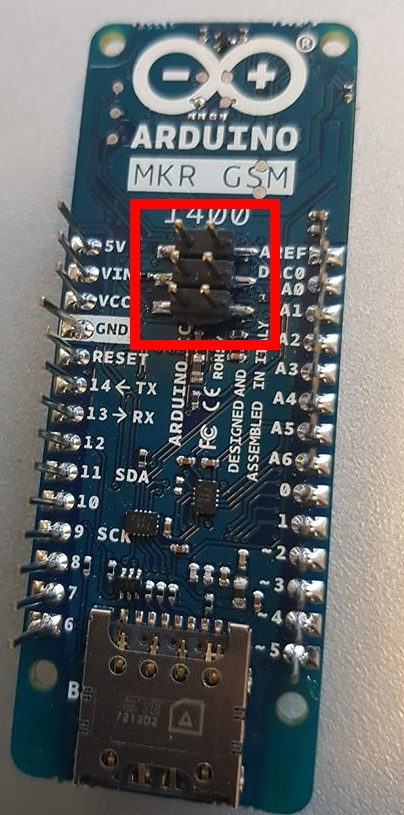
\includegraphics[height=0.4\textheight]{gfx/Implementation/MKR1400BoardSWD.jpg}
	\caption{Arduino \MKR board with SWS pins attached.}
	\label{fig:debugpins}
\end{figure}

\fxnote{GPS: e.g. Power saving settings}
\section{GSM - \SARA}
\subsection{PDP Context}
In order for the GSM module to send data packets out through GPRS, a PDP context is created through the command:
\begin{quote}
	AT+CGDCONT=1,"IP","www.internet.mtelia.dk"
\end{quote}

The command describes what packet protocol to use (IP) and the APN of the cellular network. When a context is declared and the device is registered on a network, the context can be activated. Once activated the module is assigned an ip, which will be used to send data through.

\subsection{PSD}
Creating sockets on \SARA requires a internal PDP context, also described as a PSD (Packet Switch Data) profile. This is set up similar to the external context, just with another command:
\begin{quote}
	AT+UPSD=0,1,"www.internet.mtelia.dk"
\end{quote}
Defining context 0, using 1(APN) and "www.internet.mtelia.dk" as apn. Once both context has been activated, a socket is created, in this case a UDP socket, and data can be sent to the server.

\section{GPS - \GPS}
\label{sec:impl:gps}
The location data received from the \GPS GPS is stored in a struct defined as shown in \cref{code:GPSdatat}.
The members are defined in sizes allowing the received data to be copied directly into the struct using \mintinline{c}{memcpy()}.
This is made easy as the endianness of the \GPS and the \SAMD match, both are little-endian.

\begin{listing}
	\begin{minted}[bgcolor=lightgray]{c}
struct GPS_data_t{
  uint16_t year;
  uint8_t month;
  uint8_t date;
  uint8_t hour;
  uint8_t minute;
  uint8_t second;
  uint32_t lat;
  uint32_t lon;
  // valid = 0, means data is valid.
  uint8_t valid;
};
	\end{minted}
	\caption{GPS data struct.}
	\label{code:GPSdatat}
\end{listing}

\FloatBarrier